\uuid{RI6G}
\exo7id{6981}
\auteur{blanc-centi}
\organisation{exo7}
\datecreate{2015-07-04}
\isIndication{false}
\isCorrection{true}
\chapitre{Courbes planes}
\sousChapitre{Courbes paramétrées}

\contenu{
\texte{
Représenter les courbes d'équation cartésienne $y=f(x)$, donner l'équation de 
leur tangente au point d'abscisse $x=0$ et la position de la courbe par rapport à cette tangente, pour :
}
\begin{enumerate}
    \item \question{$f(x)=\sin^2x+\cos x$}
    \item \question{$f(x)=x+\ln(1+e^x)$}
\reponse{
Pour $f(x)=\sin^2x+\cos x$, le domaine de définition de $f$ est $\R$, et 
$f$ est de classe $\mathcal{C}^\infty$. On remarque que $f$ est $2\pi$-périodique et paire, 
il suffit donc de faire l'étude de $f$ sur l'intervalle $[0;\pi]$. 
\begin{itemize}
Variations de $f$\\
Pour $x\in [0;\pi]$, $f'(x)=2\sin x\cos x-\sin x=\sin x(2\cos x-1)$ et donc $f'(x)=0$ 
si et seulement si $x\in\{0;\frac{\pi}{3};\pi\}$. Comme $\sin x>0$ si $x\in]0;\pi[$, 
pour étudier le signe de $f'(x)$, il suffit d'étudier le signe de $(2\cos x-1)$, et on obtient 
$$\begin{array}{c|lcccr}
x&0&\ &\frac{\pi}{3}&\ &\pi \\\hline
f'(x)&0&+&0&-&0\\\hline
\ &\ &\ &\frac{5}{4}&\ &\ \\
f&\ &\nearrow &\ &\searrow &\ \\
\ &1 &\ &\ &\ &-1 \\
\end{array}$$
Tangentes horizontales\\
Le graphe de $f$ possède une tangente horizontale là où $f'$ s'annule, c'est-à-dire aux points de coordonnées $(0,1)$, $(\frac{\pi}{3},\frac{5}{4})$ et $(\pi,-1)$. En particulier, la tangente au point d'abscisse 0 est horizontale et a pour équation $y=1$. Pour déterminer la position de la courbe par rapport à sa tangente en ce point, on étudie le signe de $f(x)-1$ pour $x$ proche de 0:
$$f(x)-1=\sin^2x-1+\cos x=-\cos^2x+\cos x=\cos x(1-\cos x)$$
Cette expression est positive au voisinage de $0$ (et m\^eme $>0$ pour $x\not=0$ proche de $0$). La courbe est donc au-dessus de sa tangente.
Points particuliers\\
Le graphe de $f$ coupe l'axe des abscisses entre $0$ et $\pi$ en un unique point $x_0$, qu'on détermine en résolvant
$$f(x)=0\Longleftrightarrow 1-\cos^2x+\cos x=0 \Longleftrightarrow X^2-X-1=0\ (X=\cos x)$$
ce qui donne deux solutions pour $X$, mais une seule dans $[-1;1]$: $X=\frac{1-\sqrt{5}}{2}$ et donc 
$x_0= \Arccos (\frac{1-\sqrt{5}}{2})$.
\end{itemize}
Le graphe de $f$ est obtenu sur $[-\pi;\pi]$ par symétrie par rapport à l'axe des ordonnées, 
puis sur $\R$ par $2\pi$-périodicité.

\begin{center}
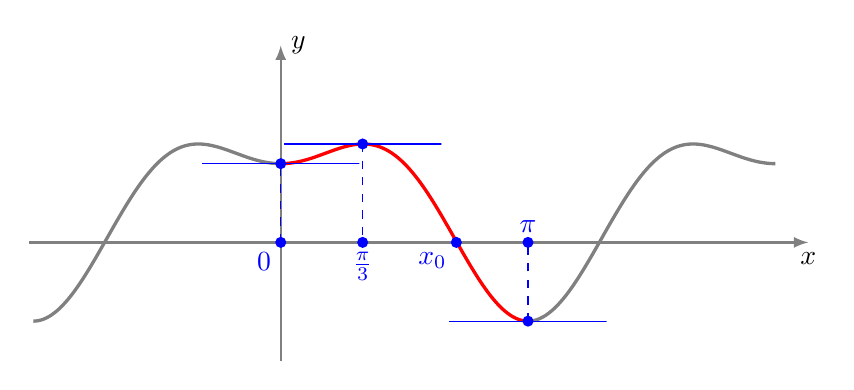
\begin{tikzpicture}[scale=1]
     \draw[->,>=latex,thick, gray] (-3.2,0)--(6.7,0) node[below,black] {$x$};
     \draw[->,>=latex,thick, gray] (0,-1.5)--(0,2.5) node[right,black] {$y$};  


  \draw[red, very thick,domain=0:pi,samples=100] plot ({\x},{sin(\x r)^2+cos(\x r)});
  \draw[gray, very thick,domain=-pi:0,samples=100] plot ({\x},{sin(\x r)^2+cos(\x r)});
  \draw[gray, very thick,domain=pi:2*pi,samples=100] plot ({\x},{sin(\x r)^2+cos(\x r)});

  \fill[blue] (2.23,0) circle (2pt) node[below left]{$x_0$};  
  \draw[blue, dashed] (0,0)--(0,1);  
  \fill[blue] (0,0) circle (2pt) node[below left]{$0$}; 
  \draw[blue, dashed] (3.14,-1)--(3.14,0);
  \fill[blue] (3.14,0) circle (2pt)  node[above]{$\pi$}; 
  \draw[blue, dashed] (1.04,1.25)--(1.04,0);  

  \fill[blue] (1.04,0) circle (2pt)  node[below]{$\frac\pi3$}; 

  \draw[blue] (0,1)--+(1,0)--+(-1,0);
  \draw[blue] (3.14,-1)--+(1,0)--+(-1,0);
  \draw[blue] (1.04,1.25)--+(1,0)--+(-1,0);
  \fill[blue] (0,1) circle (2pt); 
  \fill[blue] (3.14,-1) circle (2pt); 
  \fill[blue] (1.04,1.25) circle (2pt); 
\end{tikzpicture}
\end{center}

\begin{center}
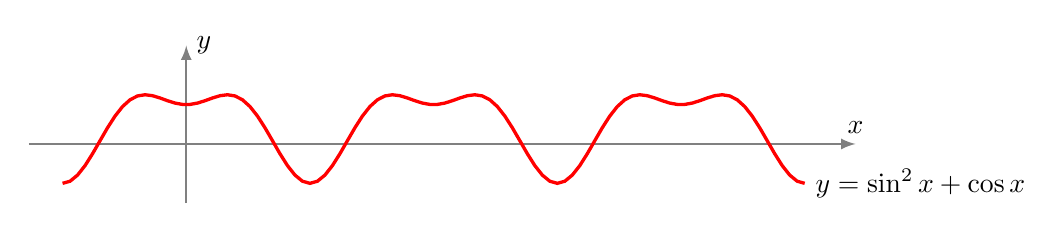
\begin{tikzpicture}[scale=0.5]
  \draw[->,>=latex,thick, gray] (-4,0)--(17,0) node[above,black] {$x$};
  \draw[->,>=latex,thick, gray] (0,-1.5)--(0,2.5) node[right,black] {$y$};  
  \draw[red, very thick,domain=-pi:5*pi,samples=100] plot ({\x},{sin(\x r)^2+cos(\x r)})
  node[black, right] {$y = \sin^2x+\cos x$};
\end{tikzpicture}
\end{center}
Pour $f(x)=x+\ln(1+e^x)$, le domaine de définition de $f$ est $\R$ et $f$ est de classe $\mathcal{C}^\infty$.
\begin{itemize}
Variations de $f$\\
Comme $f'(x)=1+\frac{e^x}{1+e^x}$, pour tout $x$, $f'(x)>1$. En particulier $f$ est strictement croissante sur $\R$.
Allure du graphe en $+\infty$\\
On a $f(x)\xrightarrow[x\to +\infty]{}+\infty$ et
$$\frac{f(x)}{x}=1+\frac{\ln\big( e^x (e^{-x}+1)\big)}{x}=1+\frac{x+\ln(e^{-x}+1)}{x}\xrightarrow[x\to +\infty]{}2$$
puis $f(x)-2x=\ln(e^{-x}+1)\xrightarrow[x\to +\infty]{}0^+$. Ainsi le graphe de $f$ a en $+\infty$ une asymptote, d'équation $y=2x$, et reste au-dessus de cette asymptote.
Allure du graphe en $-\infty$\\
On a $f(x)\xrightarrow[x\to -\infty]{}-\infty$ et
$$\frac{f(x)}{x}=1+\frac{\ln(1+e^x)}{x}\xrightarrow[x\to -\infty]{}1$$
puis $f(x)-x=\ln(1+e^{x})\xrightarrow[x\to -\infty]{}0^+$. Ainsi le graphe de $f$ 
a en $-\infty$ une asymptote, d'équation $y=x$, et reste au-dessus de cette asymptote.
Tangente au point d'abscisse $0$\\
L'équation de la tangente au graphe de $f$ au point d'abscisse $x_0$, 
et la position du graphe par rapport à cette tangente, peuvent \^etre 
obtenues simultanément à partir du développement limité de $f$ en $x_0$. 
Pour l'équation de la tangente, un développement limité à l'ordre $1$ suffit, 
mais pour avoir la position il faut pousser le développement limité à l'ordre $2$ 
(ou à l'ordre $3$ si le terme d'ordre $2$ est nul, ou plus encore...):
\begin{eqnarray*}
f(x)&=&x+\ln(1+e^x)=x+\ln\left(1+1+x+\frac{1}{2}x^2+o(x^2)\right)\\
 &=&x+\ln 2+\ln\left(1+\frac{1}{2}x+\frac{1}{4}x^2+o(x^2)\right)\\
 &=&x+\ln 2+\left(\frac{1}{2}x+\frac{1}{4}x^2\right)-\frac{1}{2}\left(\frac{1}{2}x+\frac{1}{4}x^2\right)^2+o(x^2)\\
 &=&\ln 2+\frac{3}{2}x+\frac{1}{8}x^2+o(x^2)
\end{eqnarray*}
L'équation de la tangente au point d'abscisse $0$ (donnée par le DL à l'ordre $1$) est donc 
$$y=\ln 2+\frac{3}{2}x$$ 
De plus, $f(x)-\left(\ln 2+\frac{3}{2}x\right)=\frac{1}{8}x^2+o(x^2)=\frac{1}{8}x^2(1+o(1))$
où $o(1)$ est un terme qui tend vers $0$ quand $x\to 0$. Ainsi $(1+o(1))$ a le m\^eme signe que $1$ 
pour $x$ proche de $0$, et $f(x)-\left(\ln 2+\frac{3}{2}x\right)$ est positif au voisinage de $0$: 
la courbe reste localement au-dessus de sa tangente.
\end{itemize}

\begin{center}
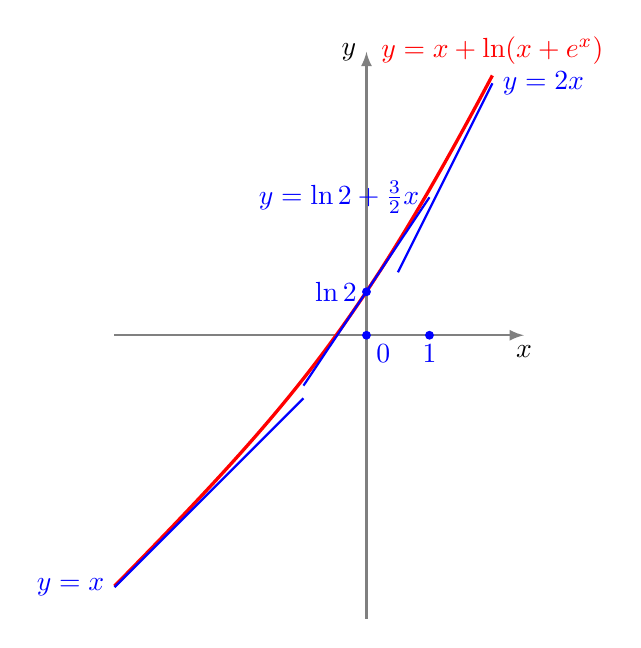
\begin{tikzpicture}[scale=0.8]

     \draw[->,>=latex,thick, gray] (-4,0)--(2.5,0) node[below,black] {$x$};
     \draw[->,>=latex,thick, gray] (0,-4.5)--(0,4.5) node[left,black] {$y$};  


  \draw[red, very thick,domain=-4:2,samples=100] plot ({\x},{\x + ln(1+exp(\x))})
  node[above] {$y=x+\ln(x+e^x)$};

  \draw[thick, blue] (-1,-1)--(-4,-4) node[left] {$y=x$};
    \draw[thick, blue] (0.5,1)--(2,4) node[right] {$y=2x$};
  \draw[thick, blue] (1,2.19)--(-1,-0.80) node[pos=0, left] {$y=\ln 2+\frac32 x$};

  \fill[blue] (0,0.69) circle (2pt)  node[left]{$\ln 2$}; 
  \fill[blue] (0,0) circle (2pt) node[below right]{$0$}; 
  \fill[blue] (1,0) circle (2pt) node[below]{$1$};
\end{tikzpicture}
\end{center}
}
\end{enumerate}
}
